% Created 2010-01-08 Fri 14:28
%\documentclass[11pt]{article}
\documentclass[pre,preprint, 11pt]{revtex4}
\usepackage[utf8]{inputenc}
\usepackage[T1]{fontenc}
\usepackage{graphicx}
\usepackage{longtable}
\usepackage{hyperref}


\title{The Impact of Beer Consumption on Scientific Collaboration}
%\author{Mario Fasold}
\date{08 January 2010}

\begin{document}

\maketitle

\setcounter{tocdepth}{3}
\tableofcontents
\vspace*{1cm}
\section{Introduction}
\label{sec-1}

\subsection{Previous Work}
\label{sec-1.1}

Some studies relating scientific output and beer have previously been done.
\begin{quote}
In Europe, most alcohol is consumed as beer and, based on well known negative effects of alcohol consumption on cognitive performance, I predicted negative correlations between beer consumption and several measures of scientific performance.
\end{quote}

\section{Results}
\label{sec-2}

\subsection{What beer should you drink}
\label{sec-2.1}

\begin{itemize}
\item Becks
\item Czech Budweiser \cite{AnMa}
\item Duff
\end{itemize}
\begin{figure}[htb]
\centerline{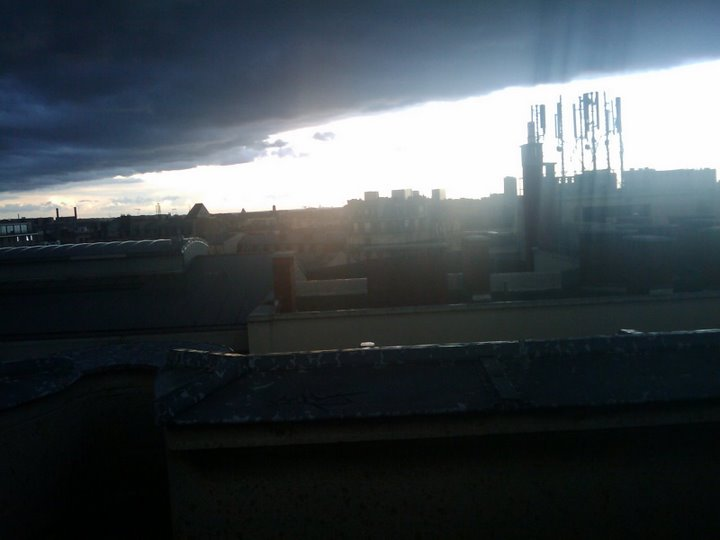
\includegraphics[scale=0.75]{./darker.jpg}}
\caption{\label{fig:degradation}Degradation Plot}
\end{figure}

\bibstyle{apsrev}
\bibliography{/home/dwblair/Dropbox/dwbdocs/physics/writing/bibfiles/dwbreferences}

\end{document}